\documentclass[12pt,a4paper]{article}
\usepackage[utf8]{inputenc}
\usepackage{amsmath}
\usepackage{amsfonts}
\usepackage{amssymb}
\usepackage{graphicx, neuralnetwork,tikz}
\usepackage{float}
\usetikzlibrary{positioning}


\input defs.tex
\bibliographystyle{alpha}
\graphicspath{ {./figures/} }
\tikzstyle{process} = [rectangle, minimum width=3cm, minimum height=1cm, text centered, draw=black]
\tikzstyle{arrow} = [thick,->,>=stealth]

\tikzstyle{state}=[shape=circle,draw=blue!30,fill=blue!10]
\tikzstyle{observation}=[shape=rectangle,draw=orange!30,fill=orange!10]
\tikzstyle{lightedge}=[<-, dashed]
\tikzstyle{mainstate}=[state, thick]
\tikzstyle{mainedge}=[<-, thick]
\tikzstyle{block} = [draw,rectangle,thick,minimum height=2em,minimum width=2em]
\tikzstyle{sum} = [draw,circle,inner sep=0mm,minimum size=2mm]
\tikzstyle{connector} = [->,thick]
\tikzstyle{line} = [thick]
\tikzstyle{branch} = [circle,inner sep=0pt,minimum size=1mm,fill=black,draw=black]
\tikzstyle{guide} = []
\tikzstyle{snakeline} = [connector, decorate, decoration={pre length=0.2cm,
                         post length=0.2cm, snake, amplitude=.4mm,
                         segment length=2mm},thick, magenta, ->]




\title{Neural Network Based Decoding over Molecular Communication Channels}
\author{Peter Hartig}
%Remove this penaltiy if hyphenation is okay. 
\hyphenpenalty=10000

\begin{document}
\maketitle

\begin{abstract}
Estimation of the distribution function characterizing a communication channel is investigated. Pilot symbol sequences may be used to estimate an unknown distribution function or when the function is difficult to parameterize. This work focuses on using pilot sequences to train a neural network and mixture model whose output supplies the necessary metrics for the Viterbi algorithm. We investigate the detection performance for estimation of non-linear channels. A proposal is then made to reduce the complexity of the resulting detection using unsuperised clustering of channel states for the Viterbi algorithm. 
\end{abstract}

\newpage
\tableofcontents
\newpage
\section{Notation}
The following notation is used throughout this work.
$p(x)$ is the probability of an event $x$.
$p(x|y)$ is the conditional probability of $x$ given $y$.
$E[x]$ is the expected value of a random variable $x$.

Vectors  are denoted by bold font ($\mathbf{x}$) and are assumed column vectors.
The vector $\mathbf{x}_{\mathrm{i}}^{\mathrm{j}}$ denotes a vector containing elements i $\rightarrow$ j of $\mathbf{x}$. $|\mathcal{A}|$ denotes the cardinality of the set $\mathcal{A}$.
$\underset{x}{\text{argmin}} \; f(x)$ is the value of variable $x$ which minimizes $f(x)$.

\section{Introduction}
Characterizing and obtaining information about the probability distribution governing communication channels is a fundamental barrier to communication. While optimal and sub-optimal strategies for overcoming this barrier have enabled vast and effective communication infrastructure, this barrier still limits communication in many contexts. One such context is the Molecular Communication channel which may be non-linear, time variant, and dependent on the specific transmitted information.
\par
Communication contexts, such as wireless, use "pilot" symbol-streams obtain channel information to parameterize a chosen channel model. The overhead of transmitting pilot sequences is, however, incompatible with the low symbol rate (and relative coherence time?) of Molecular Communication channels. The success of this data-driven technique in wireless channels suggest that perhaps an alternative, data-driven method may be successful for detection over Molecular Communication channels. One potential data-driven method for characterizing these channels is a neural network. Neural networks have shown to be an effective tool in data-driven approximation of probability distributions.
\par

The general communication channel is equivalent to a conditional probability $p(x|y)$, with transmitted information $x$ and received information $y$.  $p(x|y)$ takes into account the (potentially random) channel through which the information $x$ passes. The communication problem entails a form of the optimization $\underset{x\in\mathcal{A}}{\text{argmin}} \; p(x|y)$, in which $\mathcal{A}$ is the set of possible $x$. In general, sub-optimal solutions do not require perfect knowledge of the distribution $p(x|y)$ and may be used when the true $p(x|y)$ is unknown or impractical to obtain. This work investigates a neural network estimate of $p(x|y)$.

\section{Background}

\subsection{MLSE and the Viterbi Algoithm}
The optimization problem
\begin{equation}\label{opt_problem}
\underset{x \in \textit{$\mathcal{A}$}}{\text{argmin}} \; p(y|x),
\end{equation}
 with transmitted information $x$ and received information $y$, is also known as Maximum Likelihood Sequence Estimation (MLSE). 
The size of the search space $|\mathcal{A}|$ is grows exponentially in the length of $x$, the number of the transmitted symbols. Additional information about the communication channel can reduce the complexity of this search as illustrated in the following example.
\par
Consider the communication channel for which each received symbol in the sequence $\mathbf{y}$ is a causal, linear, and time invariant (LTI) combination of a set of the transmitted symbol sequence $\mathbf{x}$ with coeffients $\mathbf{a}$. 

\begin{equation*}
y[k] = \sum_{\mathrm{l=1}}^{\mathrm{L}} a[l]x[k-l].
\end{equation*}

In this case,
\begin{equation*}
p(\mathbf{y}|\mathbf{x})=\sum_{\mathrm{i=1}}^{\mathrm{N}}log(p(y_{\mathrm{i}}|\mathbf{x}_{\mathrm{i-L+1}}^{\mathrm{i}}) ).
\end{equation*}
Noting that terms in this sum are independent, and that the set of possible transmitted sequences $\mathbf{x}_{\mathrm{i-L+1}}^{\mathrm{i}}$ is equivalent to a set of channel states, problem \eqref{opt_problem} is equivalent finding the shortest path through a trellis  with edges weighted by $log(p(y_{\mathrm{i}}|\mathbf{x}_{\mathrm{i-L+1}}^{\mathrm{i}}))$ as in figure \ref{fig:trellis}.

\begin{figure}[H]
\begin{center}
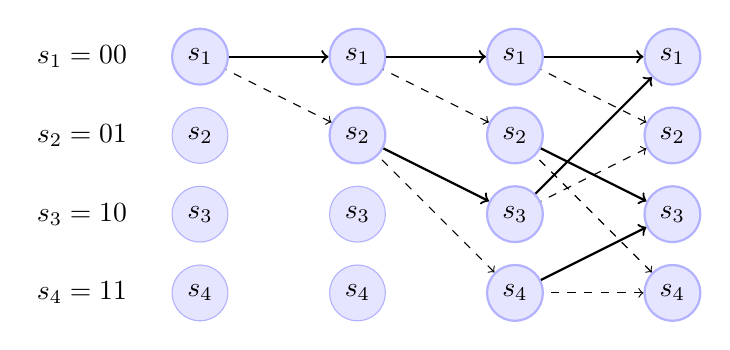
\begin{tikzpicture}[]
% 1st column
\node               at (-1.5,5) {$s_1=00$};
\node               at (-1.5,4) {$s_2=01$};
\node               at (-1.5,3) {$s_3=10$};
\node               at (-1.5,2) {$s_4=11$};
\node[mainstate] (s1_1) at (0,5) {$s_1$};
\node[state] (s2_1) at (0,4) {$s_2$};
\node[state] (s3_1) at (0,3) {$s_3$};
\node[state] (s4_1) at (0,2) {$s_4$};
%\node at (0,1) {Node1};
% 2nd column
\node[mainstate] (s1_2) at (2,5) {$s_1$}
    edge[mainedge] (s1_1);
\node[mainstate] (s2_2) at (2,4) {$s_2$}
     edge[lightedge] (s1_1);

\node[state] (s3_2) at (2,3) {$s_3$};

\node[state] (s4_2) at (2,2) {$s_4$};

%\node at (2,1) {Node2};
% 3rd column
%\node               at (4,6) {$t=2$};
\node[mainstate] (s1_3) at (4,5) {$s_1$}
    edge[mainedge]  (s1_2);

\node[mainstate] (s2_3) at (4,4) {$s_2$}
    edge[lightedge] (s1_2);

\node[mainstate] (s3_3) at (4,3) {$s_3$}
    edge[mainedge] (s2_2);    
\node[mainstate] (s4_3) at (4,2) {$s_4$}
    edge[lightedge] (s2_2);
%\node at (4,1) {Node3};
% 4th column
%\node               at (6,6) {$t=3$};
\node[mainstate] (s1_4) at (6,5) {$s_1$}
    edge[mainedge]  (s1_3)
    edge[mainedge]  (s3_3);
\node[mainstate] (s2_4) at (6,4) {$s_2$}
    edge[lightedge] (s1_3)
    edge[lightedge] (s3_3);
\node[mainstate] (s3_4) at (6,3) {$s_3$}
    edge[mainedge] (s2_3)
    edge[mainedge] (s4_3);
\node[mainstate] (s4_4) at (6,2) {$s_4$}
    edge[lightedge] (s2_3)
    edge[lightedge] (s4_3);
%\node at (6,1) {Node4};

\end{tikzpicture}
	\end{center}
	\caption{MLSE decoding for $\mathcal{A}=\{0,1\}$ and $L=2$}
	\label{fig:trellis}
\end{figure}


For finite state, causal channels, MLSE reduces to the Viterbi Algorithm over a trellis of states.
\\

    \noindent\rule[16pt]{\textwidth}{0.6pt}
	Viterbi Algorithm:

    \noindent\rule[10pt]{\textwidth}{0.4pt}
    {\footnotesize
    \begin{tabbing}
        {\bf given} $p(y_{\mathrm{i}}|x_{\mathrm{i-L+1}}^{\mathrm{i}}) \; \forall i \in {1..N}$ . \\*[\smallskipamount]
        {\bf for $i = 1..N $} \\
         \qquad \= {\bf for each state $s \in \mathcal{A}_{\mathrm{i-L+1}}^{\mathrm{i}}$}\\
        \qquad \qquad \= 1.\ Let $\textit{cost}_{s}^{\text{i}} = -log(p(y_{\mathrm{i}}|x_{\mathrm{i-L+1}}^{\mathrm{i}})) + \underset{s}{\text{min}} \{incoming\;\textit{cost}_{s}^{\text{i-1}}\}$ \\
%        \> 2.\ {\bf break if} $f(z) \leq \hat{f}_{\lambda}(z, x^{k})$. \\
%        \> 3.\ Update $\lambda := \beta \lambda$. \\*[\smallskipamount]
        {\bf return} Symbols corresponding to path of $\underset{s}{\text{argmin}} \; \textit{survivor cost}_{s} $
    \end{tabbing}}
    \noindent\rule[10pt]{\textwidth}{0.4pt}


Note that the Viterbi algorithm is \emph{exponentially} complex in the number of channel states $|\mathcal{A}_{\mathrm{i-L+1}}^{\mathrm{i}}|$, but \emph{linearly} complex in the length of the transmitted sequence $\mathbf{x}$ ($N$ in the algorithm above). 


\subsection{ViterbiNet}
Despite the reduction in complexity offered by the Viterbi Algorithm for MLSE, the individual metrics used in each step of the algorithm,
$p(y_{\mathrm{i}}|\mathbf{x}_{\mathrm{i-L+1}}^{\mathrm{i}}),$
 require knowledge of the channel probability distribution. This may be difficult or costly to obtain. Instead, we decompose using Baye's theorem,
\begin{equation*}
p(y_{\mathrm{i}}|\mathbf{x}_{\mathrm{i-L+1}}^{\mathrm{i}}) = 
\frac
{p(\mathbf{x}_{\mathrm{i-L+1}}^{\mathrm{i}}|y_{\mathrm{i}})p(y_{\mathrm{i}})}
{p(\mathbf{x}_{\mathrm{i-L+1}}^{\mathrm{i}})},
\end{equation*}
and estimate the individual terms as:

\begin{itemize}
\item $p(\mathbf{x}_{\mathrm{i-L+1}}^{\mathrm{i}}|y_{\mathrm{i}})$
: The probability of being in channel state $\mathbf{x}_{\mathrm{i-L+1}}^{\mathrm{i}}$ given the corresponding received symbol $y_{\mathrm{i}}$. If the number of states is finite, the probability mass function over $\mathbf{x}_{\mathrm{i-L+1}}^{\mathrm{i}} \in
|\mathcal{A}_{\mathrm{i-L+1}}^{\mathrm{i}}|$ can be estimated using a neural network for classification as in figure \ref{nn}. 
	\begin{figure}[H]
	\centering
		\begin{neuralnetwork}[height=4, nodespacing=10mm, layerspacing=15mm]
		\newcommand{\x}[2]{$x_#2$}
		\newcommand{\y}[2]{$\hat{y}_#2$}
		\newcommand{\hfirst}[2]{\small $h^{(1)}_#2$}
		\newcommand{\hsecond}[2]{\small $h^{(2)}_#2$}
		\newcommand{\hthird}[2]{\small $h^{(3)}_#2$}
		\newcommand{\hfourth}[2]{\small $h^{(4)}_#2$}
		\inputlayer[count=1, bias=false, title=Received\\, text=\x]
		\hiddenlayer[count=2, bias=false, title=\\, text=\hthird] \linklayers
		\hiddenlayer[count=3, bias=false, title=\\, text=\hfourth] \linklayers
		\outputlayer[count=4, title=States\\, text=\x] \linklayers
	    \end{neuralnetwork}
	    	  	  \caption{State classification Neural Network}
\label{nn}
	\end{figure}

\item $p(y_{\mathrm{i}}) = \sum_{s \in \textit{$\mathcal{S}$}}p(s,y_{\mathrm{i}})$
: The joint probability of channel state $s$ and received signal $y_{\mathrm{i}}$ marginalized over all channel states $\mathcal{S}$. For the case of the LTI channel above, each state $s$ corresponds to a possible symbol sequence $\mathbf{x}_{\mathrm{i-L+1}}^{\mathrm{i}}$. This probability distribution function can be estimated using a mixture-model (figure \ref{fig:mm}) based on training data of received signals (in this case the same data used to train the neural network) and a model for channel noise. The Expectation Maximization Algorithm \cite{ng2000cs229} is used with a chosen model for the channel states and noise. 
In the case of Gaussian noise used here, the states are modeled as a mixture of Gaussians.
%\\
%
%    \noindent\rule[16pt]{\textwidth}{0.6pt}
%	Expectation Maximization Algorithm for Gaussian Mixture Model: (TODO Discuss how much derivation is needed here)
%
%    \noindent\rule[10pt]{\textwidth}{0.4pt}
%    {\footnotesize
%    \begin{tabbing}
%        {\bf given} $p(y_{\mathrm{i}}|x_{\mathrm{i-L+1}}^{\mathrm{i}}) \; \forall i \in {1..N}$ . \\*[\smallskipamount]
%        {\bf for $i = 1..N $} \\
%         \qquad \= {\bf for each state $s$ at time $i$}\\
%        \qquad \qquad \= 1.\ Let $\textit{survivor cost}_{s}  += \text{min}\{\text{incoming transition costs}\}$ \\
%%        \> 2.\ {\bf break if} $f(z) \leq \hat{f}_{\lambda}(z, x^{k})$. \\
%%        \> 3.\ Update $\lambda := \beta \lambda$. \\*[\smallskipamount]
%        {\bf return} Symbols corresponding to path of $\underset{s}{\text{argmin}} \; \textit{survivor cost}_{s} $
%    \end{tabbing}}
%    \noindent\rule[10pt]{\textwidth}{0.4pt}
\par As $p(y_{\mathrm{i}})$ is constant over all states in a given step of the Viterbi algorithm, this term in the Baye's decomposition may be interpreted as a weighting factor for the cost of one received symbol in the total path cost. (More detail on this or enough?)


%picture of MM
%	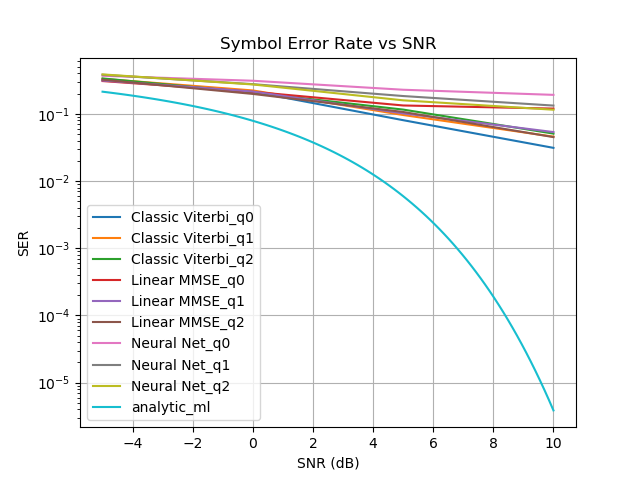
\includegraphics[width=\textwidth,height = 7cm]{results/quant_standard}

\begin{figure}[H]
\centering
	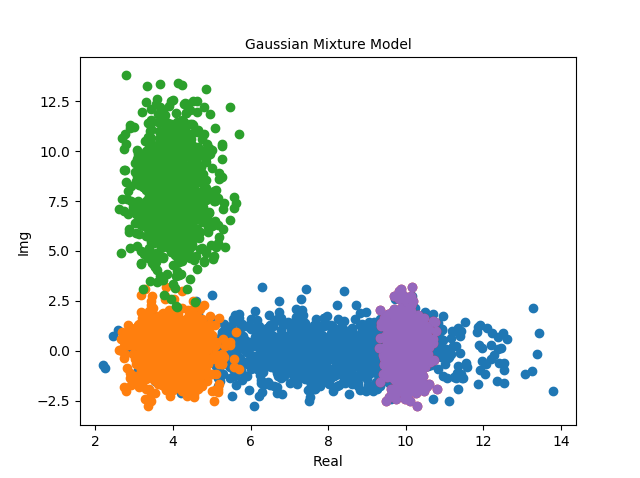
\includegraphics[width=\textwidth,height = 10cm]{system_model/mm}
	  	  \caption{Mixture of complex, Gaussian sources  }
	  \label{fig:mm}
\end{figure}

\item $p(\mathbf{x}_{\mathrm{i-L+1}}^{\mathrm{i}})$
: The probability of a given transmitted sequence can be neglected in the case of equiprobable symbols.

\end{itemize}

In summary, the metrics $p(y_{\mathrm{i}}|\mathbf{x}_{\mathrm{i-L+1}}^{\mathrm{i}})$ required by the Viterbi algorithm can be estimated using a neural network and a mixture model.





\subsection{A Reduced State ViterbiNet}
While the Viterbi Algorithm complexity scales exponentially in the number of states possible in each step of the algorithm, in some cases this complexity can be reduced without significant degradation of performance. In particular, if the system is such that some states are redundant, these can be combined. The following, relevant example with state redundancy is posed and one potential method of reducing the number of states is considered. 

Consider a received signal
\begin{equation*}
y[k] = \sum_{\mathrm{l=1}}^{\mathrm{L}} a[l]x[k-l] + n[k], \; n[k]  \sim \mathcal{N}(0,1)
\end{equation*}

with $x[k-l] \in \{ -1, +1\}$ and $n[k]  \sim \mathcal{N}(0,1)$.  

In the case of a causal, LTI system with inter-symbol-interference characterized by $\mathbf{a} = [a[1]...a[5]]=[1, 0, .2, .2, .4]$ ($\|\mathbf{a}\|^2_2 = 1$), the received signal (Fig.\ref{fig:redundant_channel}) has fewer than the potential $|\mathcal{A}_{\mathrm{i-L+1}}^{\mathrm{i}}| =2^5$ states. As one of the channel taps is 0, this will have no impact and thus 16 of the potential 32 states are removed. Further, as there are two taps of value 0.2, these together represent only 3 states rather than 4. 

%\begin{figure}[H]
%\centering
%	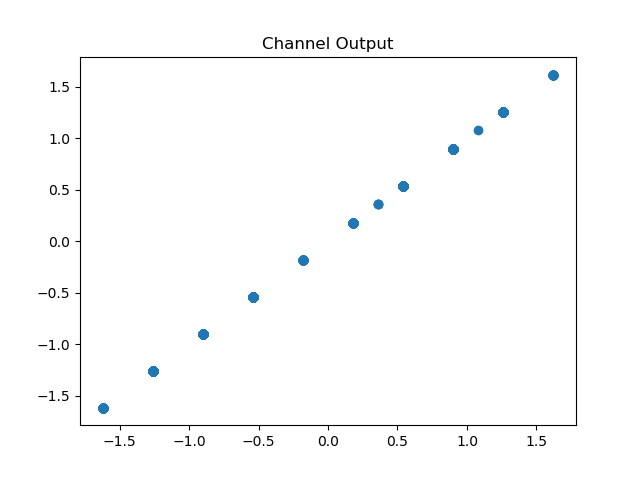
\includegraphics[width=10cm,height = 10cm]{system_model/channel_output}
%	  \label{fig:redundant_channel}
%	  	  \caption{LTI channel with state redundancy with high SNR}
%\end{figure}

One way to exploit state redundancy is to cluster the original states $|\mathcal{A}_{\mathrm{i-L+1}}^{\mathrm{i}}|$  states into a set of $k$ clusters using training data. The K-Means algorithm is proposed as one such method.
\\

    \noindent\rule[16pt]{\textwidth}{0.6pt}
K-Means Clustering Algorithm: A method for unsupervised classification

    \noindent\rule[10pt]{\textwidth}{0.4pt}
    {\footnotesize
    \begin{tabbing}
    {\bf given} initial location $L_c, \forall \;c  \in \{1..K\}$ of K centroids.\\
        {\textbf{for} Number of Iterations}.\\
         \qquad \= {\bf for each training data point $x_{\mathrm{i}}, \;\mathrm{i}  \in \{1..N\}$}\\
        \qquad \qquad \= 1.\ Label $x_i$ with the index c of the closest centroid using $\|x_{\mathrm{i}}- \text{L}_c\|^2_2$. \\
        \qquad \= {\bf for centroid $L_c, \forall \;c  \in \{1..K\}$}\\
                \qquad \qquad \= 1.\ Move $L_{\mathrm{c}}$ to the average location of all training points with label .c\\


%        \> 2.\ {\bf break if} $f(z) \leq \hat{f}_{\lambda}(z, x^{k})$. \\
%        \> 3.\ Update $\lambda := \beta \lambda$. \\*[\smallskipamount]
        {\bf return} Centroid locations.
    \end{tabbing}}
    \noindent\rule[10pt]{\textwidth}{0.4pt}
    
Choosing an appropriate number of clusters will influence the performance of the resulting decoder (Have figure showing this).
\par An implementation point to note is that after clustering the training data, the number of states must be increased by $|\mathcal{A}_{\mathrm{i}}|$. The Viterbi algorithm selects a symbol sequence corresponding to a path of state transitions through the trellis. In order to make the correspondence between a unique path and a symbol sequence, each state transition must represent a transmitted symbol. \emph{Each} resulting centroid from the k-means clustering is associated to \emph{each} potential transmit symbol in order to create a "shorter" trellis for which each state transition still represents a transmitted symbol. 

Discuss minimum phase representations for channels and why this might be an advantage. 

\subsection{The Molecular Communication Channel}
Provide necessary background for any nano-particle data shown in results. 



\section{Results}
\subsection{A supervised equalization benchmark}
The Linear Minimum Mean-Squared Error (LMMSE) equalizer derived below is used provide a linear equalization reference to the non-linearity of the proposed neural network, mixture model equalization.
\par
The convex and continuously differentiable optimization problem 

\begin{equation*}\label{mmse}
\underset{\mathbf{\mathbf{h}} \in \textit{$\mathcal{C}_{lengthx1}$}}{\text{argmin}} \;
 E[\|x-\mathbf{h}^T\mathbf{y}\|^2],
\end{equation*}\
minimizing the squared error of the linearly detected symbol $\mathbf{h}^T\mathbf{y}$ and true symbol $x$ 
is solved using
\begin{equation*}\label{mmse}
\frac{\partial  E[\|x-\mathbf{h}^T\mathbf{y}\|^2]}{\partial \mathbf{h} } = 0
\end{equation*}
to give the optimal LMMSE equalizer
\begin{equation*}\label{mmse}
\mathbf{h} = E[\mathbf{R}_{yy}]^{-1}E[\mathbf{r}_{yx}].
\end{equation*}
$E[\mathbf{R}_{yy}]$ and $E[\mathbf{r}_{yx}]$ are estimated by
\begin{equation*}\label{mmse}
 E[\mathbf{R}_{yy}]= \frac{1}{\mathrm{N}}\sum_{\mathrm{i=1}}^{\mathrm{N}}
\mathbf{y}\mathbf{y^{\mathrm{H}}} 
 \end{equation*}
 and
\begin{equation*}\label{mmse}
E[\mathbf{r}_{yx}]= \frac{1}{\mathrm{N}}\sum_{\mathrm{i=1}}^{\mathrm{N}}
\mathbf{y}x
;
 \end{equation*}
 using the same training data as the neural network and mixture model. 
Note that just as with the neural network, making this estimate requires knowledge (or estimation) of the channel memory length $L$.


\subsection{Simulation Details}
\subsubsection{System Model}
Verification and further testing of the implementation and integration of the algorithms described above is performed using the following system model.

%\begin{tikzpicture}[node distance=2cm]
%\node (start) [process] {Symbol Stream};
%\node (channel) [process, right = of start] {Channel};
%\draw [arrow] (start) -- (channel);
%
%\end{tikzpicture}

\begin{equation*}
y[k] = f(\mathbf{x}) + n[k].
\end{equation*}
With $x[k] \in \{ -1, +1\}$, independent $n[k]\sim \mathcal{N}(0,1)$ and 
\begin{equation*}
\text{SNR} = \frac{E\{|x[k]|^2\}}{\sigma^2}.
\end{equation*}

Note that each received signal $y[k] $ is potentially a function of all input symbols (assume causality?). Decoding performance for realizations of the channel function $f()$ will be evaluated. 

\subsubsection{Algorithm Parameters}
The parameters for the algorithms used in this work are detailed below.
\begin{itemize}
\item \textbf{Neural Network}
\begin{itemize}
\item Architecture: 4 layers {1, 100 (Tanh activation), 50 (relu activation), $M^L$ (Softmax $\rightarrow$ Negative Log-Likelihood)}
\item Training Data Examples: 5000
\item Neural Network Updates: Admm \cite{kingma2014adam} with step size $10^{-2}$ 
\item Batch Size: 1000 
\item Backpropogation Updates (Epochs): 900
\item Loss Function: Cross Entropy
\end{itemize}
\item \textbf{Expectation Maximization Algorithm}
\begin{itemize}
\item Training Data Examples: 5000
\item Mixture Model Source Types: Gaussian
\item Number of Sources: Number of channel states
\end{itemize}
\item \textbf{K-Means Algorithm (For Reduced State ViterbiNet)}
\begin{itemize}
\item Training Data Examples: 5000
\end{itemize}
\end{itemize}


\subsection{Simulation Results}
We first evaluate the detector performance using the Linear Time Invariant channel

\begin{equation*}
y[k] = \sum_{\mathrm{l=1}}^{\mathrm{L}} a[l]x[k-l] + n[k].
\end{equation*}
with impulse response $a[l] = ...$.
Simulation results are shown in fig \ref{fig:LTI performance}
\begin{figure}[H]
	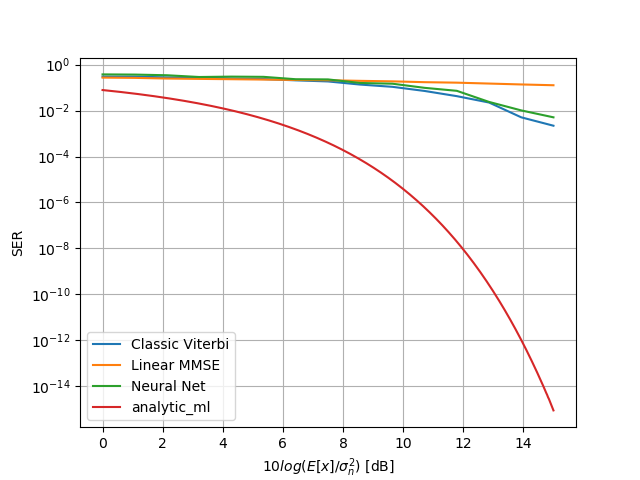
\includegraphics[width=\textwidth,height = 10cm]{results/lti_normal}
		  \caption{Detection performance over LTI channel with AWGN}
	  \label{fig:LTI performance}
\end{figure}

\subsubsection{LTI + Quantizer Channel}

To evaluate decoder performance in the non-linear channel setting, we apply a quantizer, $Q()$ to the output of the previous LTI + AWGN channel.
\begin{equation*}
y[k] = Q(\sum_{\mathrm{l=1}}^{\mathrm{L}} a[l]x[k-l]) + n[k].
\end{equation*}
 Here we evaluate performance under two levels of quantization severity: rounding channel output down to a given number of decimal places . Figure \ref{fig:Quantized Overlay} depicts the quantizer and its impact on the received symbols from the LTI channel. The resulting performance is seen in figure \ref{fig:Quantized performance}. Notice that this is essentially a reduction of the original channel states as there is now redundancy that was not previously present. 

\begin{figure}[H]
\centering
	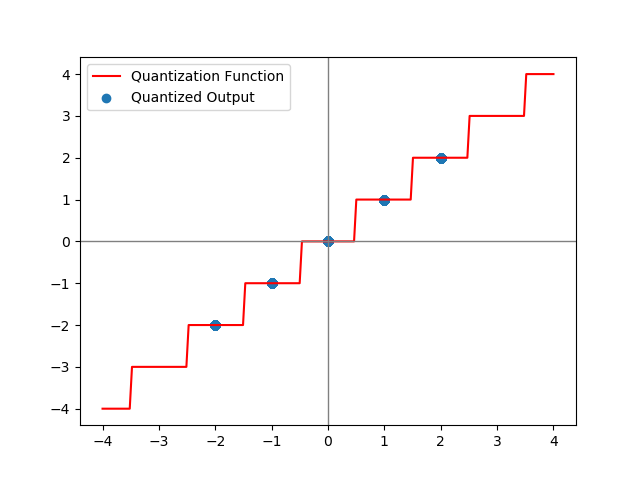
\includegraphics[width=10cm,height = 10cm]{system_model/quantizer_overlay}
			  \caption{Quantized output of LTI channel overlayed on the applied quantization function. TODO decide on axis titles }
	  \label{fig:Quantized Overlay}
\end{figure}

\begin{figure}[H]
	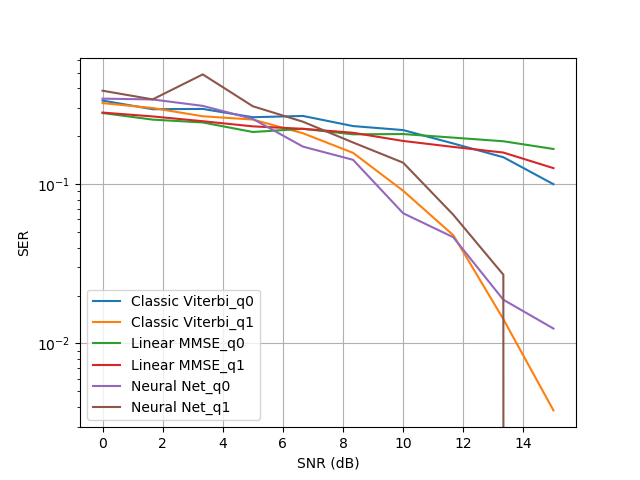
\includegraphics[width=\textwidth,height = 10cm]{results/quantized_before_noise}
		  \caption{Detection performance over LTI channel with AWGN and quantization}
	  \label{fig:Quantized performance}
\end{figure}


\subsubsection{Molecular Communication Channel}
Lastly, the performance of the neural network based detector is evaluated data collected from a molecular communication channel. ... Explain if there are any results to report. 

\section{Conclusion}
The proposed detection method from \cite{shlezinger2019viterbinet} is evaluated in  channels for which $p(y_{\mathrm{i}}|\mathbf{x}_{\mathrm{i-L+1}}^{\mathrm{i}}),$ is unknown. Simulation results indicate that this detector can indeed learn
$p(y_{\mathrm{i}}|\mathbf{x}_{\mathrm{i-L+1}}^{\mathrm{i}})$ for non-linear channels. A method for reducing the complexity of the resulting Viterbi Algorithm is also proposed, however the method of state reduction for the channel needs to be further investigated to improve the poor performance observed with the proposed method. 


\subsection{Future Work}

Extensions of specific work: 
More on reduced state.
Using other channels and repeat online type of updates for dynamic channels for these more challenging channels. 
Learning channel changes in cases for which coherence time is shorter than updates to network made by pilot symbols. 

General method extensions:
In this work the MLSE is found using the Viterbi Algorithm. The same metrics can also be used in optimizing other performance metrics. In (CITE) these estimate metrics have been used to minimize bit error rate using the BCJR algorithm. Extend to other applications of factor graphs. 

\newpage
\bibliography{report_bib}{}
\end{document}
